%=========================================================================
% Start of activity on general polynomials
%=========================================================================
\preClass{Polynomial Functions}

\begin{problem}
  \item Make a sketch of the following functions on the axes below.
    \begin{eqnarray*}
      g(x) & = & x, \\
      h(x) & = & x^2, \\
      p(x) & = & x^2+x, \\
      q(x) & = & x^3, \\
      r(x) & = & x^3+x^2.
    \end{eqnarray*}

    \begin{tikzpicture}[y=1.1cm, x=1.1cm,font=\sffamily]
        % bounds
        \def\lowX{-5.5}
        \pgfmathtruncatemacro\startX{round(0.5+\lowX)}
        \pgfmathsetmacro\nextXValue{int(\startX+1)}
        \def\highX{5.5}
        \def\lowY{-5.5}
        \def\highY{5.5}
        \pgfmathsetmacro\nextYValue{int(\lowY+1)}
        % ticks
        \draw[step = 1, gray, very thin,dashed,opacity=0.85] (\lowX, \lowY) grid ( \highX,\highY);
      % axis
      \draw[thick,->] (\lowX,0) -- coordinate (x axis mid) (\highX,0) node[anchor = north west] {$x$};
        \draw[thick,->] (0,\lowY) -- coordinate (y axis mid) (0,\highY) node[anchor = south east] {$y$};
        \foreach \y in {-5,-4,...,-1,1,2,...,\highY} {
          \draw (1pt, \y) -- (-1pt, \y) node[yshift=-6,xshift=-1,anchor=east] {$\y$};
        }
        \foreach \x in {-5,-4,...,-1,1,2,...,\highX} {
          \draw (\x,1pt) -- (\x,-1pt) node[yshift=-5,xshift=-1,anchor=east] {$\x$};
        }
        \draw (0,6.0) node [anchor=south] {Comparing Polynomials};
      \end{tikzpicture}

\end{problem}


\actTitle{Polynomial Functions}
\begin{problem}
\item For each polynomial below state its leading our term.  Also,
  determine its long term behaviour. As $x$ gets very large and
  positive what happens to the function? As $x$ gets very negative
  what happens to the function?
  \begin{subproblem}
  \item ${\displaystyle 4x^3 - 7x^2 + 5x + 8 }$.
    \vfill
  \item ${\displaystyle -7 x^6 + 3,000 x^5 + 7x^4 + x^3 - 8x^2 + 10x - 500}$.
    \vfill
  \item ${\displaystyle - \frac{1}{10} x^7 + 10,000 x^6 - 1 }$.
    \vfill
  \item ${\displaystyle \frac{1}{1000} x^{10} - 500 x^9 + 3 x^8 - 5 x^4 + 100 }$.
    \vfill
  \end{subproblem}

  \clearpage

\item Make a rough sketch of the function of the function
  \begin{eqnarray*}
    k(x) & = & -3(x+2)(x-1)(x-4)
  \end{eqnarray*}
  using the axes below.

  \begin{tikzpicture}[y=1.1cm, x=1.1cm,font=\sffamily]
    % bounds
    \def\lowX{-5.5}
    \pgfmathtruncatemacro\startX{round(0.5+\lowX)}
    \pgfmathsetmacro\nextXValue{int(\startX+1)}
    \def\highX{5.5}
    \def\lowY{-5.5}
    \def\highY{5.5}
    \pgfmathsetmacro\nextYValue{int(\lowY+1)}
    % ticks
    \draw[step = 1, gray, very thin,dashed,opacity=0.85] (\lowX, \lowY) grid ( \highX,\highY);
    % axis
    \draw[thick,->] (\lowX,0) -- coordinate (x axis mid) (\highX,0) node[anchor = north west] {$x$};
    \draw[thick,->] (0,\lowY) -- coordinate (y axis mid) (0,\highY) node[anchor = south east] {$y$};
    \foreach \y in {-5,-4,...,-1,1,2,...,\highY} {
      \draw (1pt, \y) -- (-1pt, \y) node[yshift=-6,xshift=-1,anchor=east] {$\y$};
    }
    \foreach \x in {-5,-4,...,-1,1,2,...,\highX} {
      \draw (\x,1pt) -- (\x,-1pt) node[yshift=-5,xshift=-1,anchor=east] {$\x$};
    }
    \draw (0,6.0) node [anchor=south] {The polynomial $k(x)$};
  \end{tikzpicture}

  \vfill

  \clearpage
  
\item Make up a polynomial that is strictly positive on the intervals
  $(-\infty,-4)\cup(-2,3)$
  and is strictly negative on the intervals
  $(-4,-2)\cup(3,\infty)$.

    \vfill

  \item A polynomial is strictly positive on the intervals
    $(-5,-3)\cup(-3,1)\cup(4,6)$ and is negative on the intervals
    $(-\infty,-5)\cup(1,4)\cup(6,\infty)$. What is the minimum degree
    of the polynomial?

    \vfill

    \clearpage
    
  \item  The graph of a polynomial is shown below.  Determine one
    possible formula for the polynomial.

    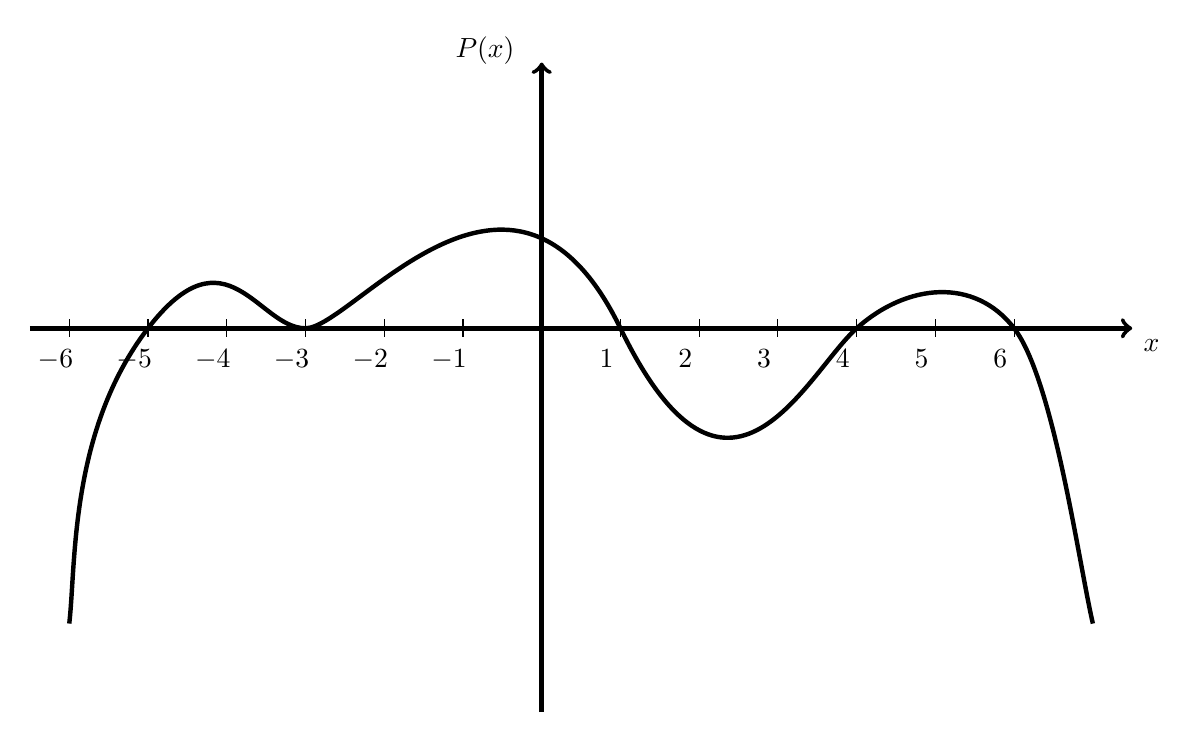
\begin{tikzpicture}[y=0.75cm, x=1.0cm,font=\sffamily]
      \begin{scope}[shift={(0,0)}]
        % axis
        \draw[ultra thick,->] (-6.5,0) -- coordinate (x axis mid) (7.5,0)
            node[anchor = north west] {$x$}; 
        \draw[ultra thick,->] (0,-6.5) -- coordinate (y axis mid) (0,4.5) 
            node[anchor = east,shift={(-0.2,0.2)}]  {$P(x)$};

      \draw[ultra thick,black]
       (-6, -5) .. controls +( 85:1)   and +(240:2)    .. (-5, 0)
       (-5,  0) .. controls +( 60:2)   and +(180: 0.6) .. (-3, 0)
       (-3,  0) .. controls +(  0:0.6) and +(110: 4.0) .. ( 1, 0)
       ( 1,  0) .. controls +(290:4.0) and +(230: 1.0) .. ( 4, 0)
       ( 4,  0) .. controls +( 50:1.0) and +(120: 1.0) .. ( 6, 0)
       ( 6,  0) .. controls +(300:1)   and +(100: 1)   .. ( 7,-5)
       ;

       \foreach \x in {-6,-5,...,-1,1,2,...,6} {
          \draw (\x,0.15) -- (\x,-0.15) node[yshift=-1,xshift=-5,anchor=north] {$\x$};
        }


    \end{scope}

    \end{tikzpicture}

    
    \vfill


\end{problem}

\postClass

\begin{problem}
\item Briefly state two ideas from today's class.
  \begin{itemize}
  \item 
  \item 
  \end{itemize}
\item 
  \begin{subproblem}
    \item
  \end{subproblem}
\end{problem}


%%% Local Variables:
%%% mode: latex
%%% TeX-master: "../labManual"
%%% End:

